\chapter{自蒸馏单目深度估计框架}
\section{引言}
作为场景感知领域中至关重要的任务,单目深度估计在近些年取得了
长足的进步,现有的单目深度估计算法大多关注估计精度与运算速度,
随着卷积神经网络(CNN)和大数据技术的迅速发展,机器可以学习到
从2D到3D无约束的映射,Saxena等人\cite{saxena2006learning}
第一次将深度学习方法应用到单目深度估计任务中,众多基于
学习的方法涌现出来\cite{DABC,xu2018structured,chakrabarti2016depth,
bts,2015semantic,lee2019monocular,godard2017unsupervised},其中
包括有监督,半监督和无监督方法。这些工作在单一场景或单一数据分布上
都取得了具有竞争力的结果,但是对交叉场景的泛化能力关注较少。
例如估计算法在室外场景
上表现良好,但是在室内场景的表现不尽如人意,反之亦然。
为了解决这个问题,本文使用复合数据集,即室内数据集(NYU depth)加
室外数据集(KITTI)来训练网络,但是当前算法在面对这些联合数据集
时都出现了不同程度的退化现象,参见图\ref{train_once_problem}。
这说明复杂多样的数
据分布给网络的
泛化能力和表达能力带来了巨大的挑战。为了解决这个问题
本章提出了一种自蒸馏单目深度估计框架,来同时学习复杂多样
例如室内、室外的数据分布。方法使用了两个共享权重的
学生编码器(Student Encoder)
分别提取两个数据集的特征,然后引入了相异性损失(Dissimilarity 
Loss) 来拉开不同数据集在特征空间上的距离。最后采用解码器
来将不同的特征上采样为最终的预测深度图,此过程受到对应数据集的
真实标注所引导。该框架为端到端的框架,可以适用任何编解码结构的
网络。
\begin{figure}[htb]
    \centering
    \begin{subfigure}{0.55\textwidth}
    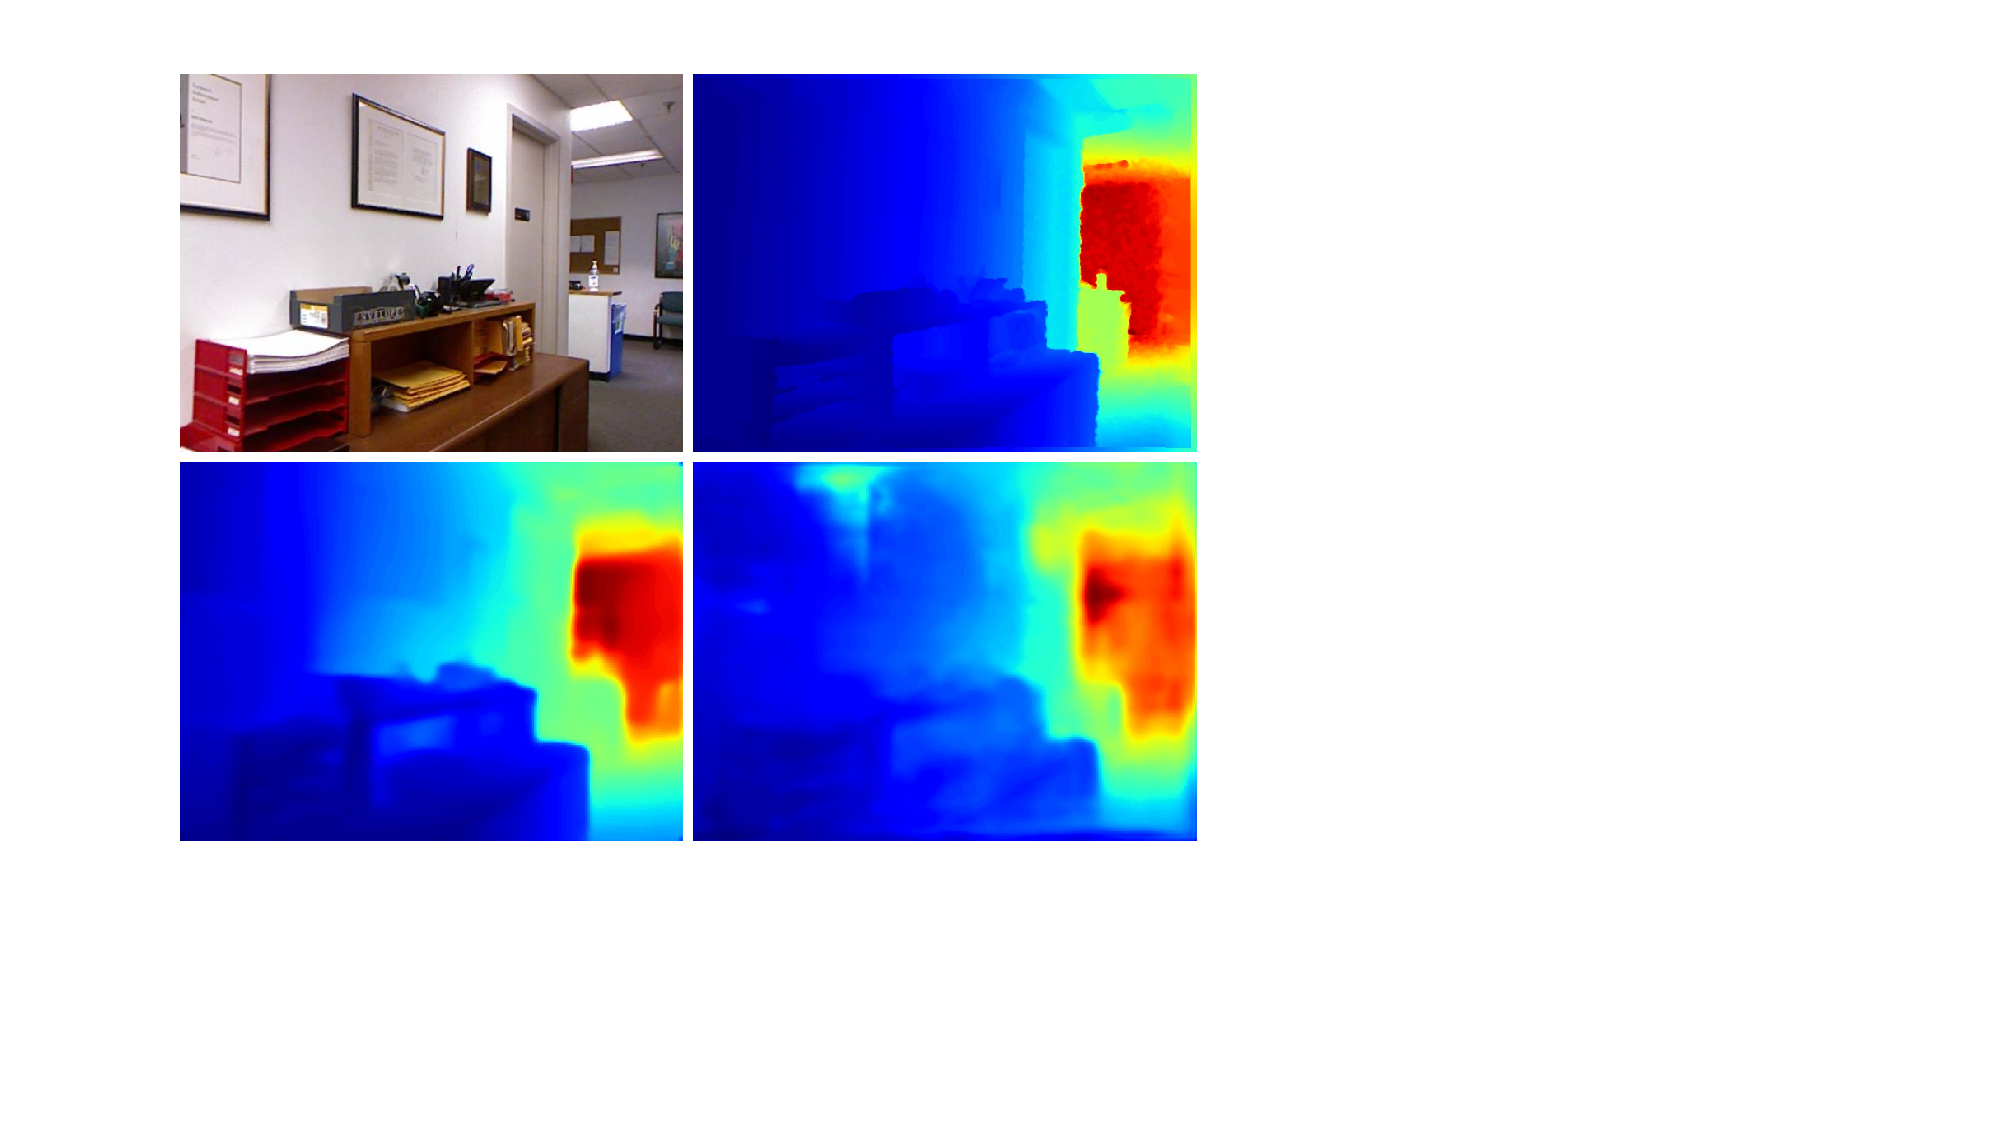
\includegraphics[width=0.95\linewidth]{figure/nyu_class_fail.pdf}
    \caption{}
    \end{subfigure}
    \begin{subfigure}{0.36\textwidth}
    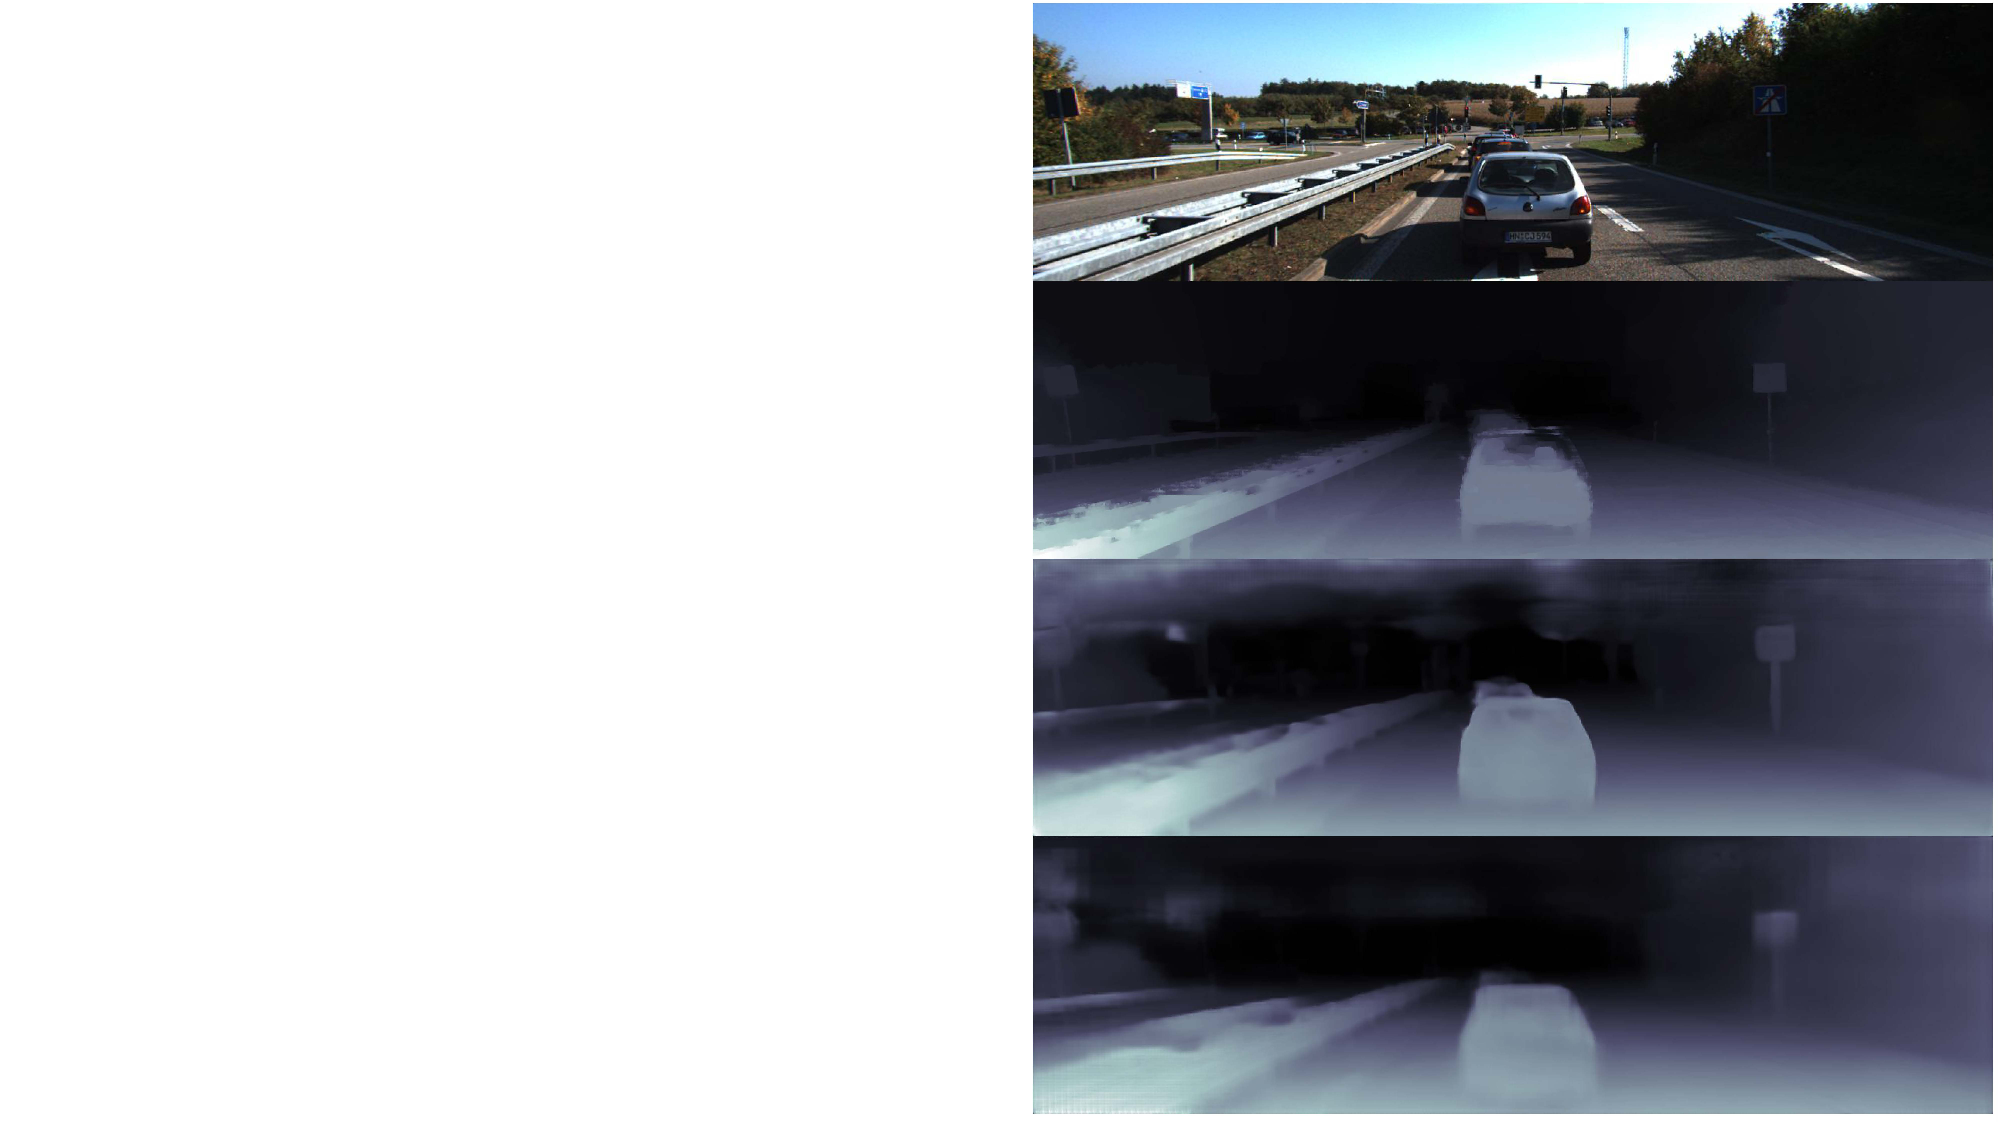
\includegraphics[width = 0.95\linewidth]{figure/kitti_bts_fail.pdf}
    \caption{}
    \end{subfigure}
    \caption{图(a)左上:RGB图像,右上:真实深度标注,左下:Li\cite{DABC}在NYU
    depth数据集上训练的预测图,右下:Li\cite{DABC}在联合数据集上训练的预测图。
    图(b)从上到下依次为:RGB图像,真实标注,BTS\cite{bts}在KITTI数据集
    上训练后的预测图,BTS\cite{bts}在联合数据集上训练的预测图。}
  \label{train_once_problem}
 \end{figure}
本章的创新点总结如下:
\begin{enumerate}
    \item 创新性地使用联合数据集
    来对网络进行训练测试,关注到了网络在对交叉场景的拟合和泛化能力。
    \item 提出了一种自蒸馏单目深度估计框架,一定程度上减弱了网络在面对复杂多样
    的数据分布时出现的性能退化现象,这种框架适用于所有的编解码网络,具有很强的移植性。
    \item 对比实验表明提出的框架对网络的拟合能力、泛化能力有了很大的提升。
\end{enumerate}

\section{自蒸馏单目深度估计框架}
\subsection{问题建模}
给定一个训练集 $\mathcal{T} = \{I,D\}$,
$I\in \mathcal{I}$, $D\in \mathcal{D}$,其中$\mathcal{I}$ 
和$\mathcal{D}$分别代表RGB图像集合和真实深度标注集合。
单目深度估计算法旨在得到RGB图像到深度图的映射:
$\varPhi:\mathcal{I}\rightarrow \mathcal{D}$。
当训练集包含复杂数据分布时
$\mathcal{T_{IO}} = \{(I_{in},I_{out}), (D_{in},D_{out})\}$,
其中$I/D_{in}$和$I/D_{out}$分别表示室内数据集和室外数据集。
算法需要强大的表达能力和拟合能力。

\begin{figure}[t]
    \centering
  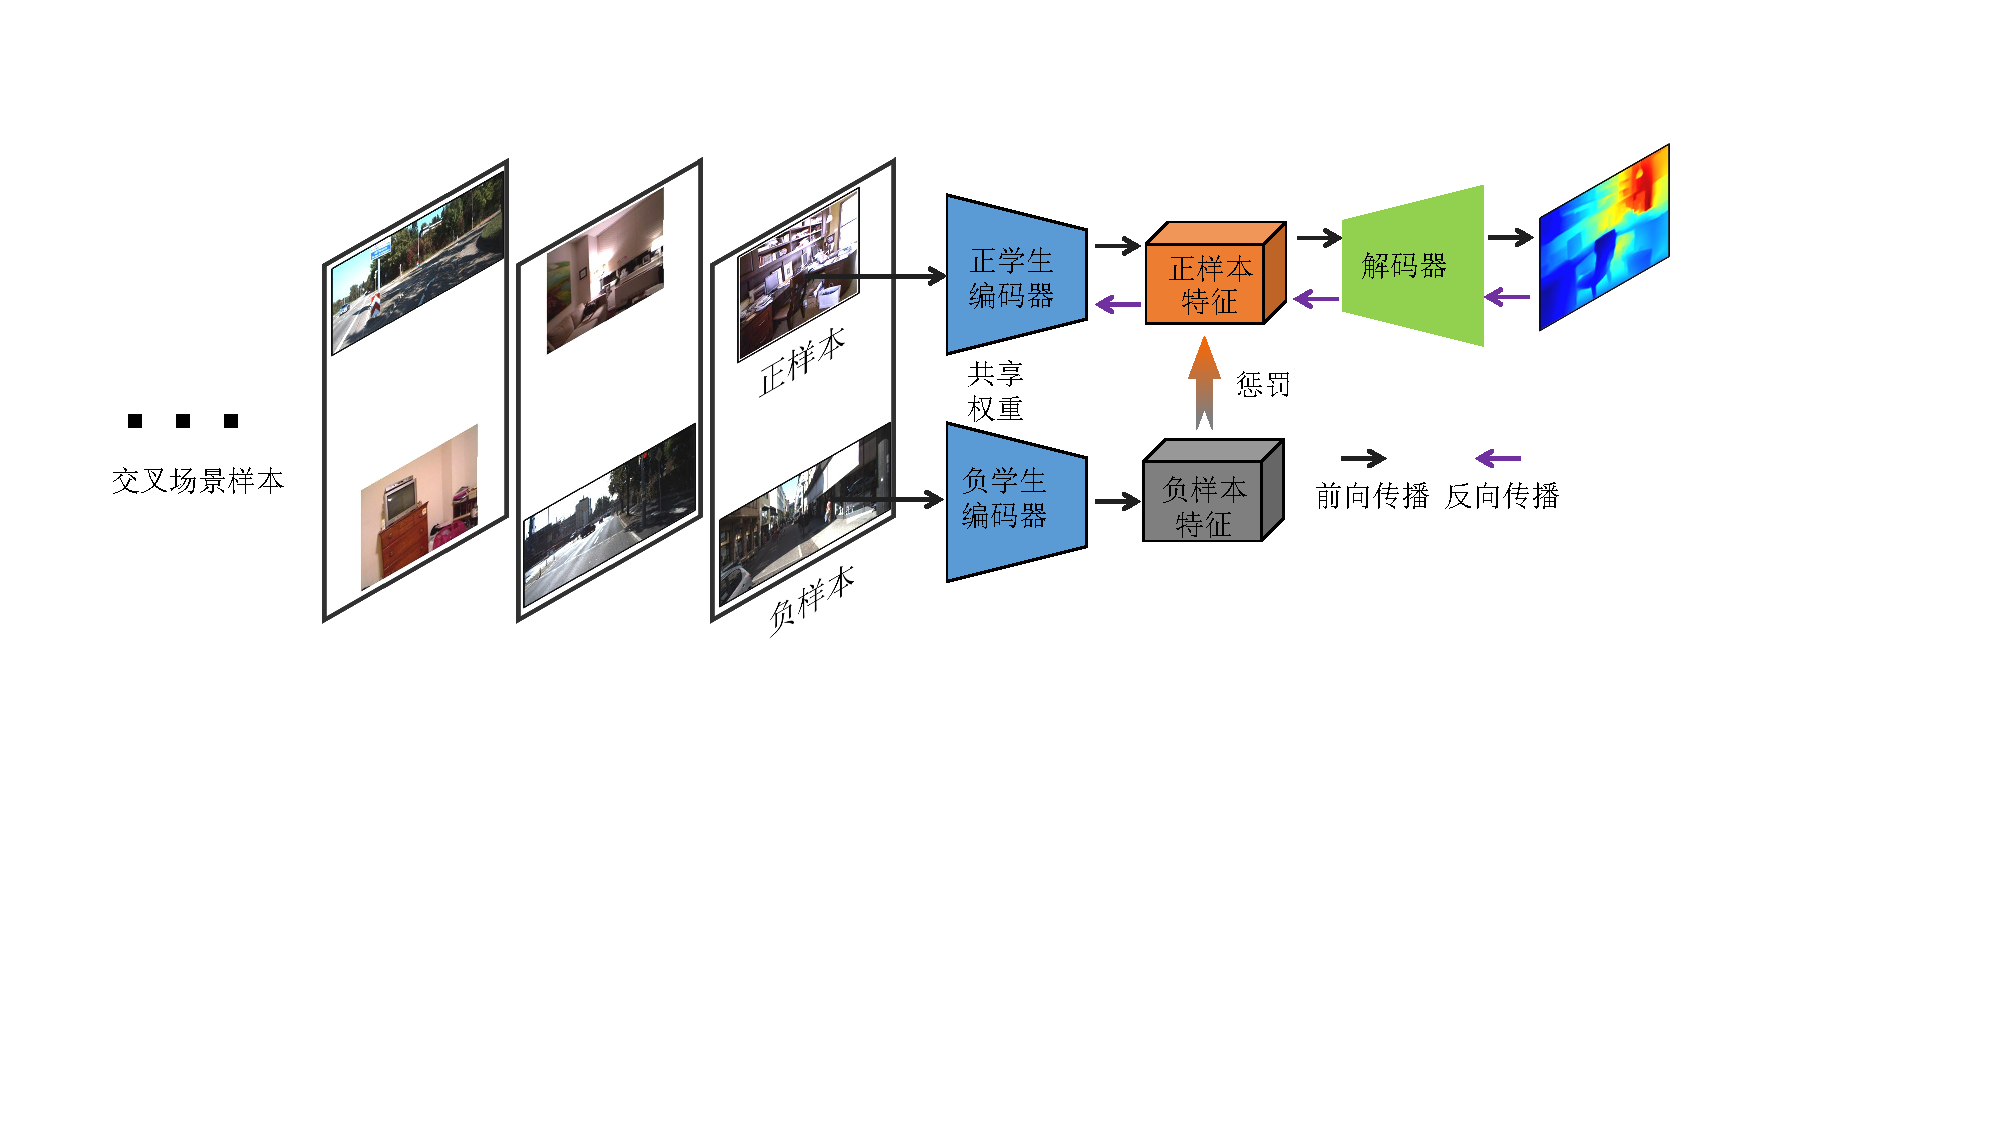
\includegraphics[width=1\linewidth]{figure/Stream.pdf}
  \centering
       \caption{针对复杂场景的自蒸馏深度估计框架}
   \label{Stream of algorithm} 
  \end{figure}
\subsection{网络结构}
\begin{algorithm*}[tbh]
  \caption{自蒸馏单目深度估计训练框架工作流程}
  \KwSty{需要训练的参数:}

      初始化KITTI参数:$\alpha$,
      NYU参数: $\beta$。
      
      \While{ $\alpha$ 或 $\beta$ 没有收敛} 
      {从KITTI或NYU数据集中随机采样一批图像

        \If(){采样了一批KITTI数据}{
          同时采样一批NYU数据\\
        \KwIn{将KITTI数据送入正学生编码器}
        通过优化损失函数$\mathcal{L}_{scale-invariant}$更新$\alpha$\\
        \KwIn{NYU数据被送入负学生编码器。}
        通过优化损失函数$\mathcal{L}_{dissimilarity}$来扩大
        $\beta$与$\alpha$之间的距离。
        }
        \If(){采样了一批NYU数据}{
          同时采样一批KITTI数据。\\
        \KwIn{将NYU数据送入正学生编码器}
        通过优化损失函数$\mathcal{L}_{scale-invariant}$更新$\beta$\\
        \KwIn{将KITTI数据被送入负学生编码器。}
        通过优化损失函数$\mathcal{L}_{dissimilarity}$来扩大
        $\alpha$与$\beta$之间的距离。
        }
      }
  \label{alg:backbone_alg}
  \end{algorithm*}
为了使算法可以更加鲁棒,首先构造了联合数据集(NYU depth和KITTI),
寄希望于算法在包含复杂场景的数据集下训练时,可以在复杂场景下
表现优异。但是随之而来的退化现象对网络的表达和拟合能力均是
一个挑战。
本章为了解决这种退化现象,采用了不同于以往的简单训练策略。
受到知识蒸馏网络的启发,设计了一种自蒸馏框架,
如图\ref{Stream of algorithm}所示。
框架同时从两个数据集分别进行采样,
正学生编码器提取正样本特征,同时负学生编码器提取另一数据集采样
的负样本的特征,负样本特征对正样本特征进行“惩罚”,
使$\mathbf{X_{IO}}$逐渐分化:
$\mathbf{X_{IO}} = \{\mathbf{X_{in}},\mathbf{X_{out}}\}$,
其中$\mathbf{X_{IO}}$代表包含室内特征和室外特征的复杂数据集。

本章采用目前最先进的算法之一BTS~\cite{bts}来实现编码器和解码器。
骨干网络采用了密集特征提取网络,得到了三个尺度
的特征图,它们的宽和高
分别为原尺寸1/2, 1/4, 1/8,随后最小的特征图经过了空洞空间金字塔模块
(Atrous Spatial Pyramid Pooling,ASPP),模块
空洞率分别为[3,6,12,18,24]。经过空洞空间金字塔池化模块
后,多尺度的语义信息被提取出来。随后每个尺度的特征图都
经过带有平面引导层
(Local Planar Guidance)的解码器,恢复为输入图原尺寸大小。
最后使用卷积层将不同尺度的预测图连接在一起计算出最终预测图。
本章设计了相异性损失函数Dissimilarity Loss使负样本对正样本进行“惩罚”,
从而使两个数据集的特征距离扩大。而该损失函数需要的特征向量需要
具有相同的尺寸,所以在编码器的最后一层,设计了
自适应池化层(Adaptive Pooling Layer)。
在经过自适应池化层之前,KITTI样本特征尺寸为$44\times88$,
而NYU depth样本特征尺寸为$52\times68$,
经过自适应池化层后他们的尺寸被统一调整为$44\times68$。
\begin{figure}[t]
    \centering
  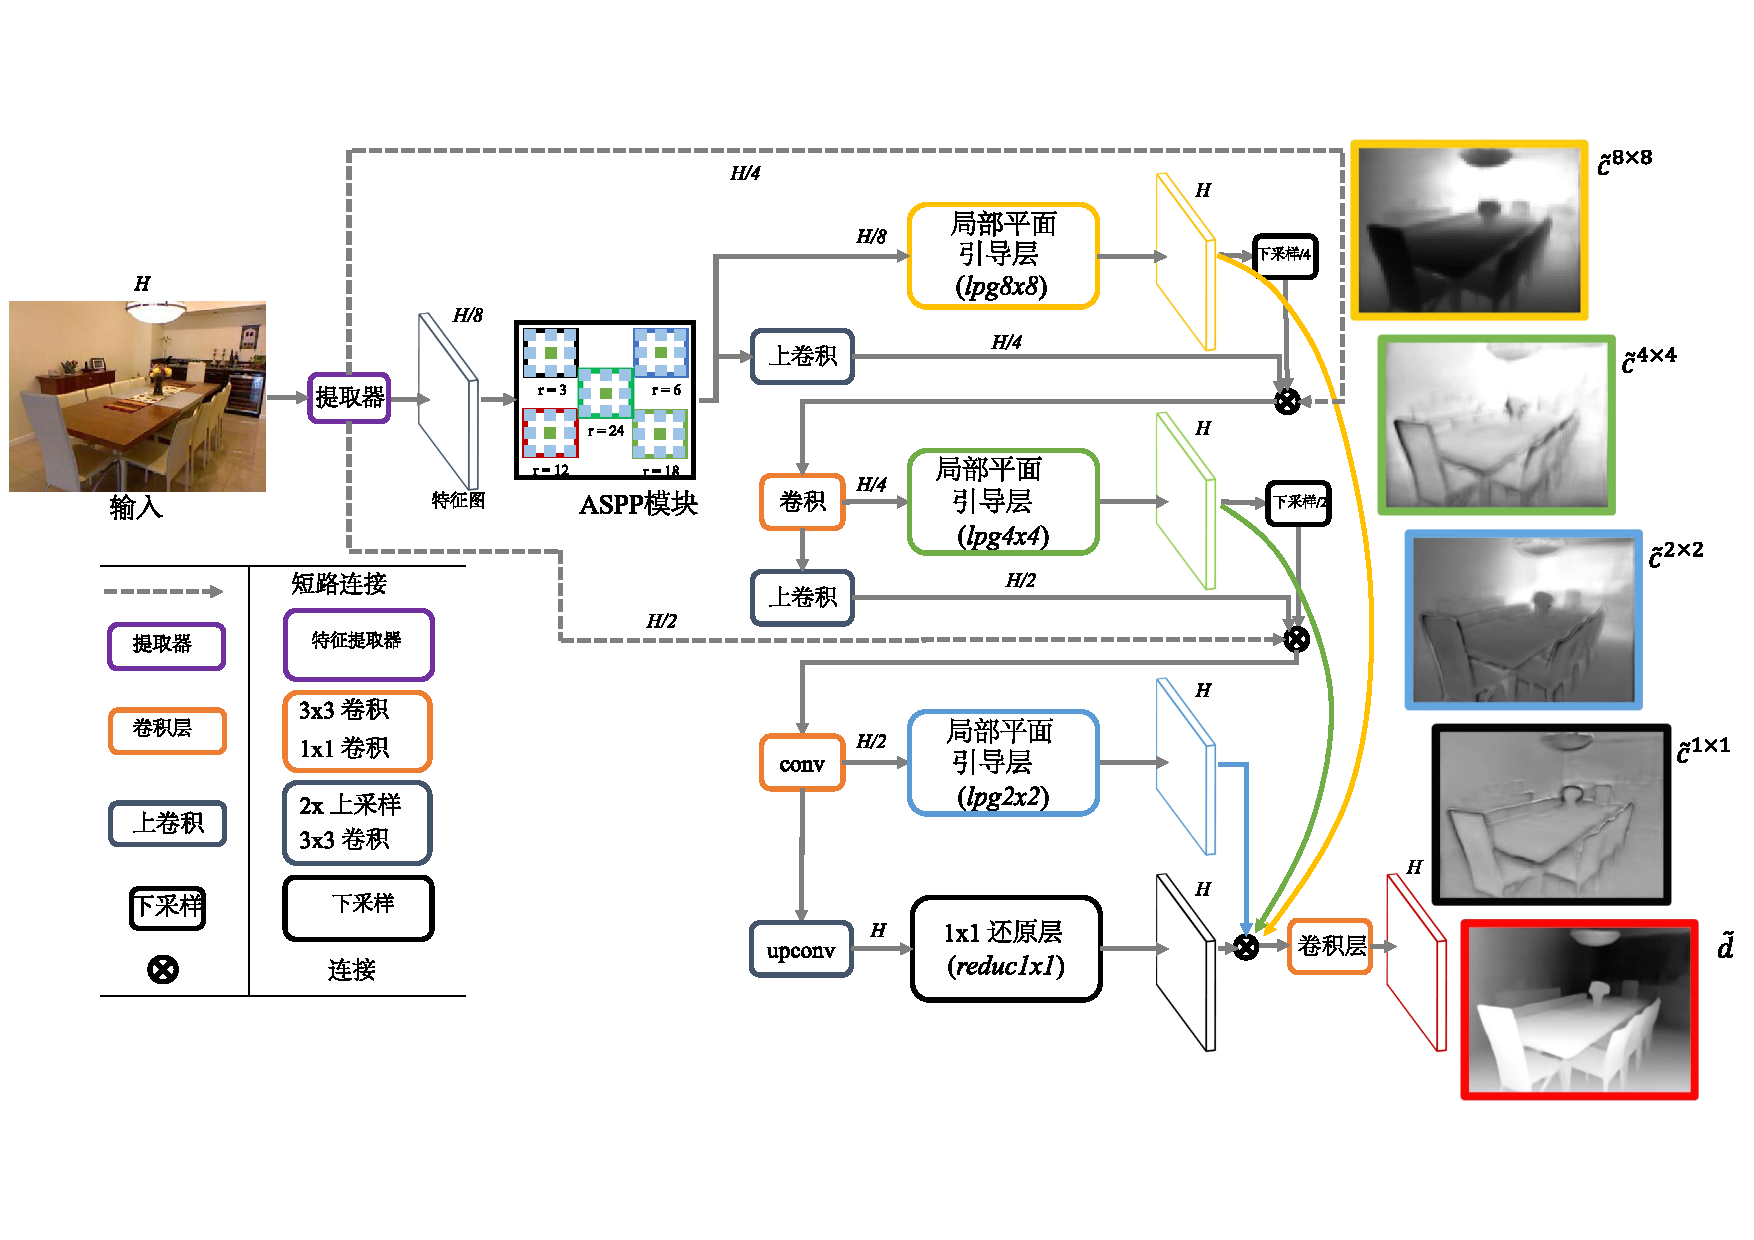
\includegraphics[width=1\linewidth]{figure/Bts_architecture.pdf}
  \centering
       \caption{自蒸馏框架使用的编解码器结构,采用了BTS\cite{bts}网络}
   \label{BTS architecture} 
  \end{figure}
 \subsection{损失函数}
一方面网络需要拟合两个数据集,另一方面网络又需要对两个
数据集进行区分,所以框架设计了两个损失函数,总的损失函数是两个
子损失函数项的线性加权。

学生编码器用来缩小相同数据集的类内间距,它由尺度一致性损失函数
\cite{eigen2014depth}来约束:
\begin{align}
  \mathcal{L}_{scale-invariant} = \frac{1}{N}\sum_{i}g_i^2-\frac{\lambda}{N^2}(\sum_{i}g_i)^2
\end{align}
其中$g_i=\log d_i^*-\log d_i$, $d_i^*$和$d_i$代表真实深度与
预测深度。$N$代表所有的像素数目。最后采用了BTS\cite{bts}
中的损失函数,因为BTS\cite{bts}证明了将损失函数的值域归一到一定范围
对预测效果有积极作用:
\begin{align}
 \mathcal{L}_{scale-invariant} = \alpha\sqrt{\frac{1}{N}\sum_{i}g_i^2-\frac{\lambda}{N^2}(\sum_{i}g_i)^2} 
\end{align}
$\alpha$在实验中被设置为10。

网络针对不同的彩色图产生相应的深度图,对网络的泛化性能
同样提出了要求。所以本章设计了$\mathcal{L}_
{dissimilarity}$来使网络对不同的数据集有所区分。
负学生编码器与正学生编码器共享权重,它
利用一组对应的样本,计算出负样本的
特征,这些特征通过dissmilarity loss的惩罚机制,不断扩大两个数据集
之间的类外间距: 
\begin{align}
  \mathcal{L}_{dissimilarity}=max(0,cos(\mathbf{x_f}, \mathbf{x_{nf}}) - margin)
\end{align} 
式中$margin$是一个系数并且在实验中设置为0。
$\mathbf{x_{f}}$和$\mathbf{x_{nf}}$分别代表正学生编码器与
负学生编码器计算的特征。
$cos(\mathbf{x_f}, \mathbf{x_{nf}})$代表两个特征图
的余弦相似性。实验中使用了$\mathbf{x_{f}}$ and $\mathbf{x_{nf}}$
沿通道维度的向量来计算余弦相似性。 

总的损失函数如下式所示:
\begin{align}
\mathcal{L} = \mathcal{L}_{scale-invariant} + \mathcal{L}_{dissimilary}
\end{align}
%(multiple means two here specially since we want our 
%subdatasets 
%contain same quality level images,so we discard
%Make3D~\cite{Make3D},
%which contains
%534 images and its images are too little to compare
%with KITTI~\cite{geiger2013vision} and NYU depth v2~\cite{Silberman:ECCV12}) at once with a semi-supervised way.

\section{实验结果与分析}
本节设计了几个实验来表明自蒸馏深度估计框架带来的提升。
包括与其他关键方法的直观衡量指标对比,与可视化结果对比。
除此之外,由于复杂数据集对单目深度估计网络的
表达能力和拟合能力都提出了新的要求,本节还通过
可视化卷积层的相关性来证明对表达能力和拟合能力的提升。
\subsection{实现细节}
\begin{figure*}[t]
  \centering
  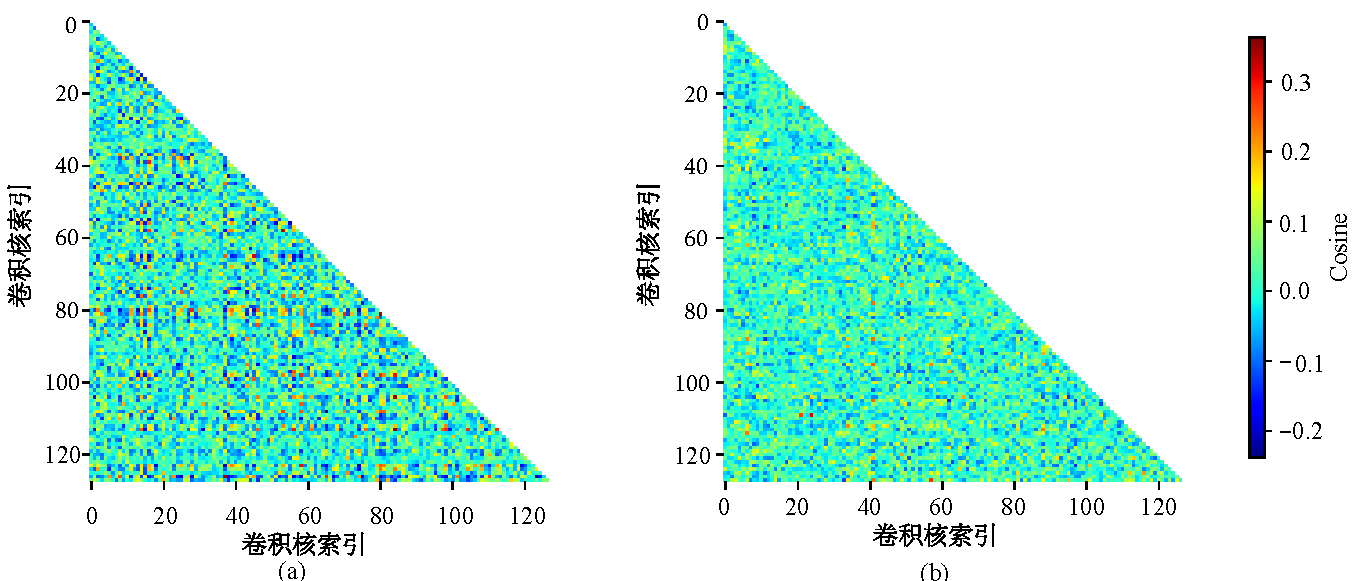
\includegraphics[width=0.85\linewidth]{figure/conv_co.pdf}
  \caption{编码器最后一层卷积核各通道之间的余弦相似性。
(a)为使用BTS~\cite{bts}采用常规训练框架时的卷积核通道相似性,
(b)为使用本章提出的自蒸馏框架训练的卷积核通道相似性。绿色代表
相似性越低。}
  \label{fig:conv_co}
  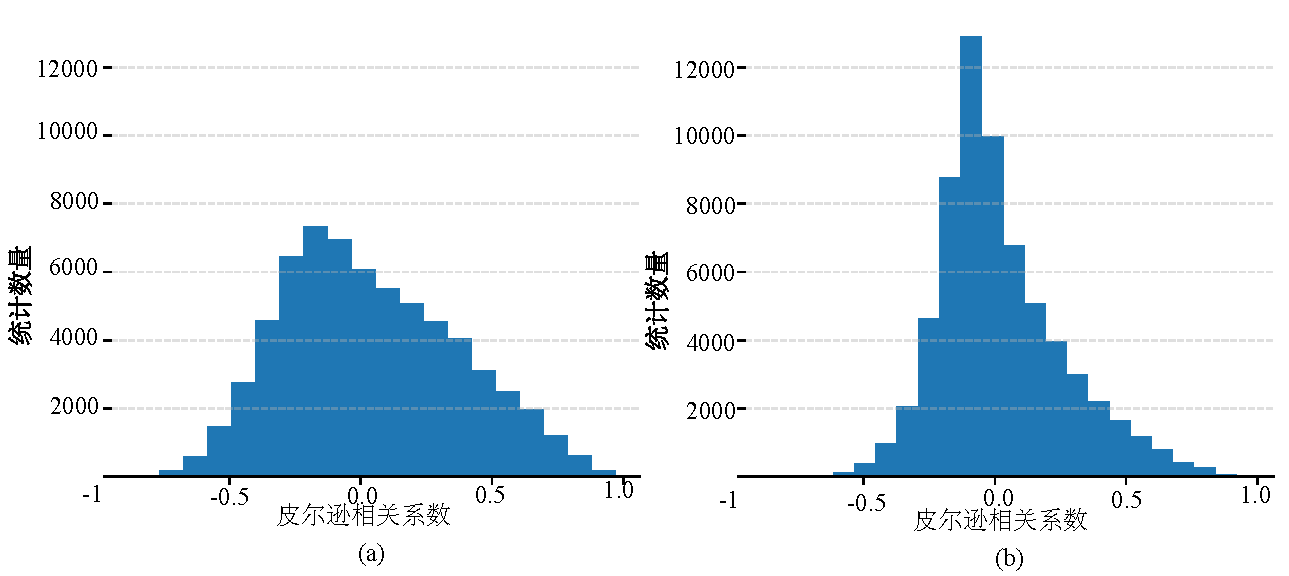
\includegraphics[width=0.85\linewidth]{figure/fea_co.pdf}
  \caption{特征图个通道间的皮尔逊相关系数的统计直方图,
  采用了[-1,-0.5],[-0.5,0],[0,0.5],[0.5,1]
  四个统计区间。(a)为使用常规训练框架训练得到的特征图的统计图,
  (b)为使用提出的自蒸馏框架训练得到的特征图的统计图。}
  \label{fig:fea_co}
\end{figure*}
本节所有实验的批尺寸均设置为4,并且设置了80000次迭代。因为KITTI
与NYU的图片同时被采样,也就是在同一批中,
但是两种数据的尺寸并不相同,其中NYU$416\times544$,KITTI
$352\times704$,所以需要将NYU图像进行左填充,将KITTI
图像进行右填充,是他们的尺寸同为$416\times704$,然后在送入网络之前,
在通过切片操作将其还原为各自尺寸。
数据增广方面,采用了与BTS~\cite{bts}相同的增广方法,
在对比度,光照,色彩调节方面,使用了范围在[0.9,1.1]
的随机调整。针对KITTI数据应用了[-2.5,2.5]的随机旋转操作,
针对NYU数据应用了[-1,1]的随机旋转操作。
整个实验实现使用了PyTorch~\cite{paszke2019pytorch}框架来完成。
\subsection{数据集与评价体系}
单目深度估计算法在室内场景和室外场景都应具有很强的鲁棒性。
然而,之前的工作一次只关注到一个场景,例如
在室外场景进行训练后测试,室内场景同理。
本章提出的算法旨在提升单目深度估计算法在室内外复杂场景
的鲁棒性,为了达到这个目的,本节在实验时组织了多个数据集,包括
室内数据集NYU depth和室外数据集KITTI。这两个数据集分别是
单目深度估计在室内场景和室外场景最常用的数据集。另外,
两个数据集包含的样本数量大致相当,相比之下Make3D和ScanNet
样本量太少,不适用于本章提出方法。

NYU depth v2数据集包含464个使用微软Kinect拍摄得室内场景
深度范围0到10m,根据Eigen\cite{eigen2014depth},实验中
从249个训练场景中选取了17000张图片以及其对应的深度图来构成
实验数据集。在测试部分仍然使用了官方发布的稠密标注测试集。
为了加速训练过程,对图像进行裁剪到$416 \times 544$。

KITTI数据集包含多个子任务数据集:物体检测,语义分割,深度估计,
深度补全等。这些子任务都是自动驾驶任务中的重点难点。深度信息和
彩色图像分别使用装载在行驶的车辆上的激光雷达与摄像机采集。
与现有工作一样,实验选取了22600张图像与对应点云组成复杂数据集。
点云在训练前使用补全方法进行了深度补全。KITTI图片被
裁剪为$352 \times 704$随后被送入网络。

为了客观公正的比较本章提出的框架,同时使方法对性能的提升有更直观的
体现,同样选取了五个广泛使用的指标\cite{eigen2014depth}:$
 RMSE=\sqrt{\frac{1}{\lvert N \rvert} \sum\nolimits_{i\in N}\lvert|d_i - d_i^*\rvert|^2} 
$,
$
  RMSE \ log = \sqrt{\frac{1}{\lvert N \rvert}\sum\nolimits_{i\in N}\lvert| \lg(d_i) - \lg(d_i^*) \rvert|^2}
$,
$
  Abs \ Rel=\frac{1}{\lvert N \rvert}\sum\nolimits_{i \in N}\frac{\lvert d_i - d_i^* \rvert}{d_i^*}
$,
$
  Sq \ Rel=\frac{1}{\lvert N \rvert}\sum\nolimits_{i \in N}\frac{\lvert| d_i - d_i^* \rvert|^2}{d_i^*}
$,
$
  Accuracies:\% \ of \ d_i \ s.t. \max(\frac{d_i}{d_i^*},\frac{d_i^*}{d_i})=\delta < thr 
$。
其中$d_i$和$d_i^*$表示预测深度与真实深度。$N$代表
所有的有效像素。 
\subsection{定量结果}

\begin{table*}[htb]
  \centering
  \caption{自蒸馏单目深度估计框架在NYU数据集的表现对比,最优结果使用加粗处理。}
  \label{tab:nyu quantitative result}
  \zihao{-5}
  \begin{tabular}{c|cc|cccc|ccc}
    \toprule
    \multirow{2}{*}{方法} & \multicolumn{2}{c|}{数据集}& \multicolumn{4}{c}{数值越低效果好}&\multicolumn{3}{|c}{数值越高效果越好}\\
    &KITTI&NYU& Rel Abs & Rel Sq & RMSE& RMSE $log$ &$\delta<1.25$ &$\delta<1.25^2$ & $\delta<1.25^3$ \\   
    \midrule
    Saxena\cite{Make3D}&&$\surd $&0.349&-&
    1.214&-&0.447&0.745&0.897\\
    Eigen\cite{eigen2014depth}&&$\surd$&0.215&-
    &0.907&0.282&0.702&0.898&0.967\\
    Liu\cite{liu2015learning}&&$\surd$&0.213&-&0.759&-&0.650&0.906&0.976\\
    Chakrabarti\cite{chakrabarti2016depth}&&$\surd$&0.149&-&0.620&-&0.806&0.953&0.988\\
    Laina\cite{laina2016deeper}&&$\surd$&0.114&0.898&4.935&0.206&0.861&0.949&0.976\\
    Lee\cite{lee2019monocular}&&$\surd$&
    0.131&0.087&0.538&-&0.837&0.971&0.994\\
    Fu\cite{FuCVPR18-DORN}&&$\surd$&0.115&-&0.509&-&0.828&0.965&0.992\\
    Xu\cite{xu2018structured}&&$\surd$&0.125&-&0.593&-&0.806&0.952&0.986\\
    \hline
    Li\cite{DABC}&&$\surd$&0.124&&0.597&0.366&0.814&0.960&0.988\\
    Li\cite{DABC}&$\surd$&$\surd$&0.174&-&0.796&0.401&0.724&0.911&0.942\\
    \hline
    BTS\cite{bts}&&$\surd$&\textbf{0.110}&-&0.392&\textbf{0.047}&\textbf{0.885}&\textbf{0.978}&\textbf{0.994}\\
    BTS\cite{bts}&$\surd$&$\surd$&0.172&0.101&0.402&0.198&0.731&0.933&0.984\\
    Ours&$\surd$&$\surd$&0.163&\textbf{0.091}&\textbf{0.388}&0.190&0.746&0.941&0.987\\
    \bottomrule
  \end{tabular}
\end{table*}
本节使用Eigen\cite{eigen2014depth}在KITTI与NYU测试数据集上
测试了提出的框架。注意实验使用组合复杂数据集进行训练,随后使用
各自的测试集对网络进行测试。在表
\ref{tab:nyu quantitative result}中使用领域关键方法
作为基准,包括
Eigen\cite{eigen2014depth},Liu\cite{liu2015learning}, 
Chakrabarti\cite{chakrabarti2016depth}, 
Laina\cite{laina2016deeper}, Lee\cite{lee2019monocular}等方法。
通过对比发现,当使用复合数据集进行训练时,Li\cite{DABC}与
BTS\cite{bts}均有不同程度的退化现象。在Rel Abs指标上
分别有40\%和56\%的衰退。单数据集表现上,BTS\cite{bts}
在大多数指标上都取得了最优的结果。当使用复杂数据集时,应用了
自蒸馏深度估计框架可以使所有指标均获得一定的提升,其中
Rel Sq, RMSE指标分别获得10\%和3\%的提升后甚至超越了在单数据集
上的表现,达到了最优效果。在正确估计像素的占比上,该框架同样
可以减缓面对复杂数据集的衰退现象。


\begin{table*}[htb]
  \centering
  \caption{自蒸馏单目深度估计框架在KITTI数据集表现对比,最优结果使用加粗处理。}
  \label{tab:kitti quantitative result}
  \zihao{-5}
  \begin{tabular}{c|cc|cccc|ccc}
    \toprule
    \multirow{2}{*}{方法} & \multicolumn{2}{c|}{数据集}& \multicolumn{4}{c|}{数值越低效果越好}&\multicolumn{3}{c}{数值越高效果越好}\\
    &KITTI&NYU& Rel Abs & Rel Sq & RMSE& RMSE $log$ &$\delta<1.25$ &$\delta<1.25^2$ & $\delta<1.25^3$ \\   
    \midrule
    Saxena\cite{Make3D}&$\surd $&&0.280&3.012&
    8.734&0.361&0.601&0.820&0.926\\
    Eigen\cite{eigen2014depth}&$\surd$&&0.203&
    1.548&6.307&0.282&0.702&0.898&0.967\\
    Liu\cite{liu2015learning}&$\surd$&&0.201&1.584&6.471&0.273&0.680&0.898&0.967\\
    Kuznietsov\cite{kuznietsov}&$\surd$&&0.113&0.741&4.621&0.189&0.862&0.960&0.986\\

    Godard\cite{godard2017unsupervised}&$\surd$&&0.114&0.898&4.935&0.206&0.861&0.949&0.976\\
    Zhow\cite{zhou2017unsupervised}&$\surd$&&
    0.198&1.836&6.565&0.275&0.718&0.901&0.960\\
    Fu\cite{FuCVPR18-DORN}&$\surd$&&0.072&0.307&\textbf{2.727}&0.120&0.932&0.984&0.994\\
    Xu\cite{xu2018structured}&$\surd$&&0.122&0.897&4.677&-&0.818&0.954&0.850\\
    \hline
    Li\cite{DABC}&$\surd$&&0.144&0.528&4.470&0.197&0.845&0.961&0.984\\
    Li\cite{DABC}&$\surd$&$\surd$&0.231&0.655&7.096&0.259&0.734&0.891&0.921\\
    \hline
    BTS\cite{bts}&$\surd$&&\textbf{0.059}&\textbf{0.245}&2.756&\textbf{0.096}&\textbf{0.956}&\textbf{0.993}&\textbf{0.998}\\
    BTS\cite{bts}&$\surd$&$\surd$&0.114&0.392&3.257&0.142&0.892&0.989&\textbf{0.998}\\
    Ours&$\surd$&$\surd$&0.115&0.389&3.036&0.144&0.890&0.989&\textbf{0.998}\\
    \bottomrule
  \end{tabular}
\end{table*}
表\ref{tab:kitti quantitative result}展示了框架在KITTI数据集
上的表现。实验同样选取了Li\cite{DABC}与BTS\cite{bts}作为
对比基准。两种方法的各个指标当使用复杂数据集时也出现了不同程度的衰退。
这再一次证明了常规方法在面对复杂数据分布时的不足。
Fu\cite{FuCVPR18-DORN}在RMSE指标上取得了最优的效果,
但是在其他指标上,BTS\cite{bts}取得了最优的结果。本章提出的框架
未能使任何指标反超BTS\cite{bts}在面对单一KITTI时的表现,但是在
$\delta<1.25^3$指标上与单一数据集的表现达到了持平。

\subsection{视觉效果}

面对特定的场景,鲁棒的单目深度估计算法可以生成特定精准的深度图,
本章方法针对不同的场景可以提取不同的特征图。
但是网络的表达能力同样扮演了重要的角色,因为
网络需要从提取的密度特征来生成最终的深度图。
本节计算了自适应池化层之前的卷积层各通道之间的
余弦相似性。图\ref{fig:conv_co}表明本框架可以降低网络卷积通道之间
的相关性,从而降低卷积核的冗余性。但是图(a)表明,在复杂数据集上的
常规训练方式使得网络仍然具有很强的冗余性,进而降低了网络的表达能力。
实验还计算了编码器产生的特征图通道之间的皮尔逊相关系数
(Pearson Correlation Coefficient, PCC)。
具体计算方式如下:特征图具有128个通道,将特征图的
长、宽维度展开,使其尺寸变为$128\times\mathbf{(H\times W)}$,
随后计算了特征图每个通道之间的皮尔逊相关系数,如图
\ref{fig:fea_co}所示。 与简单的使用复杂数据集训练相比,
本章自蒸馏框架产生的特征图通道之间的皮尔逊相关系数更多的集中在0
附近,即具有更少的相关性。但是图(a)中展示的统计图,
通道之间的相关性较为分散,具有较强的相关性,即特征图
并没有被很好的分化。

\begin{figure*}[htb]
  \centering
  \begin{subfigure}{0.15\linewidth}
  \begin{minipage}[b]{1\linewidth}
  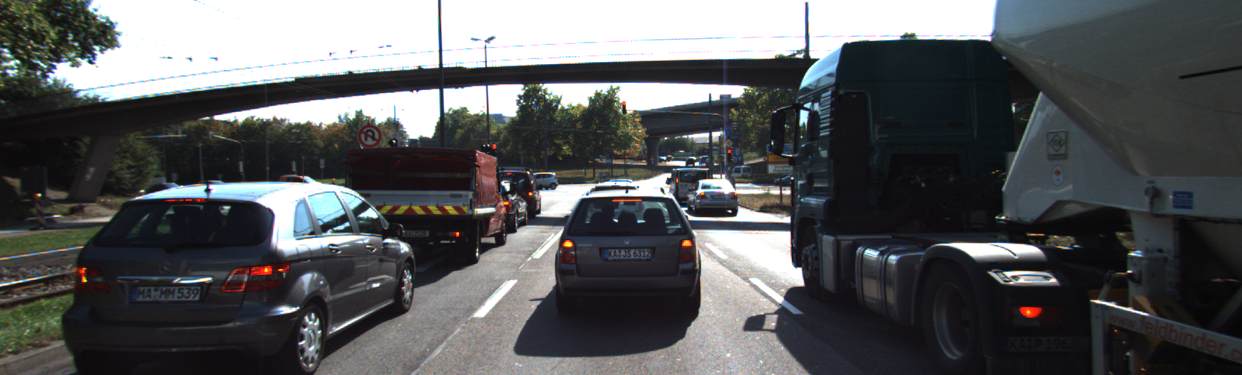
\includegraphics[width=1\linewidth]{figure/kitti_rgb/0000000000.png}\vspace{4pt}
  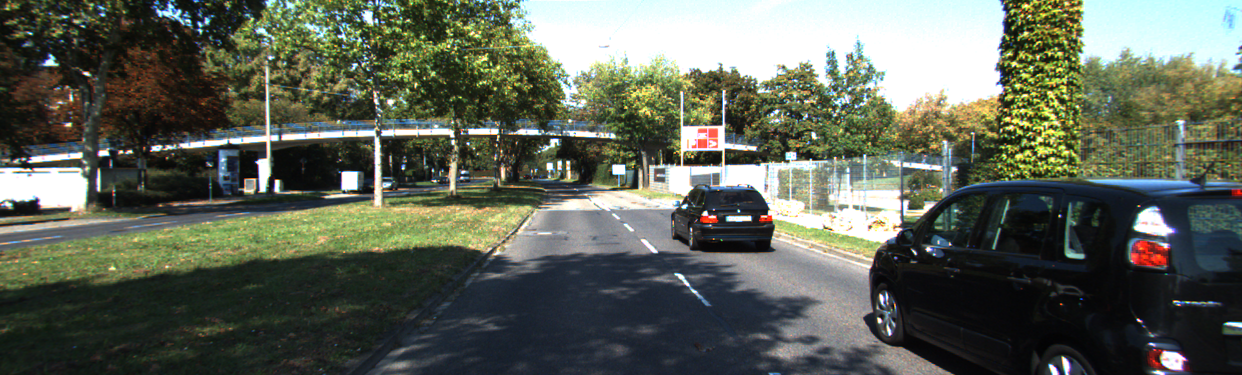
\includegraphics[width=1\linewidth]{figure/kitti_rgb/0000000035.png}\vspace{4pt}
  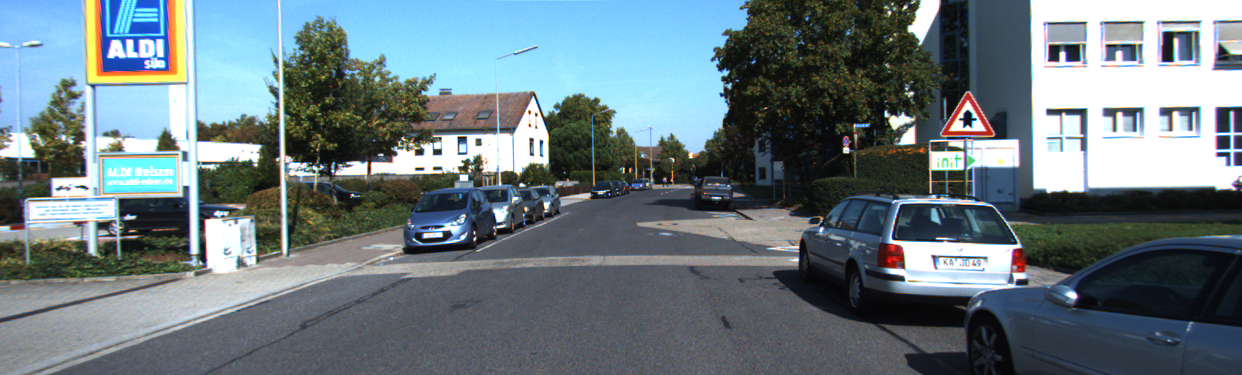
\includegraphics[width=1\linewidth]{figure/kitti_rgb/0000000260.png}\vspace{4pt}
  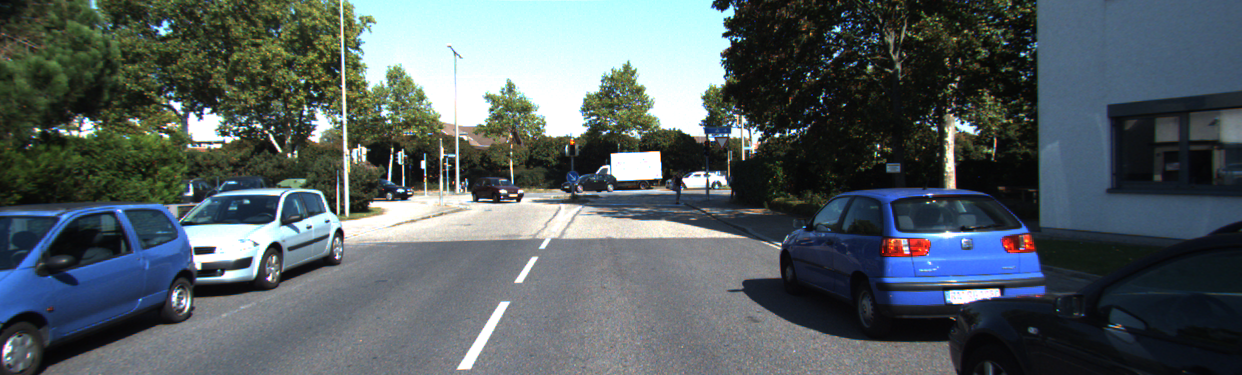
\includegraphics[width=1\linewidth]{figure/kitti_rgb/0000000340.png}\vspace{4pt}
  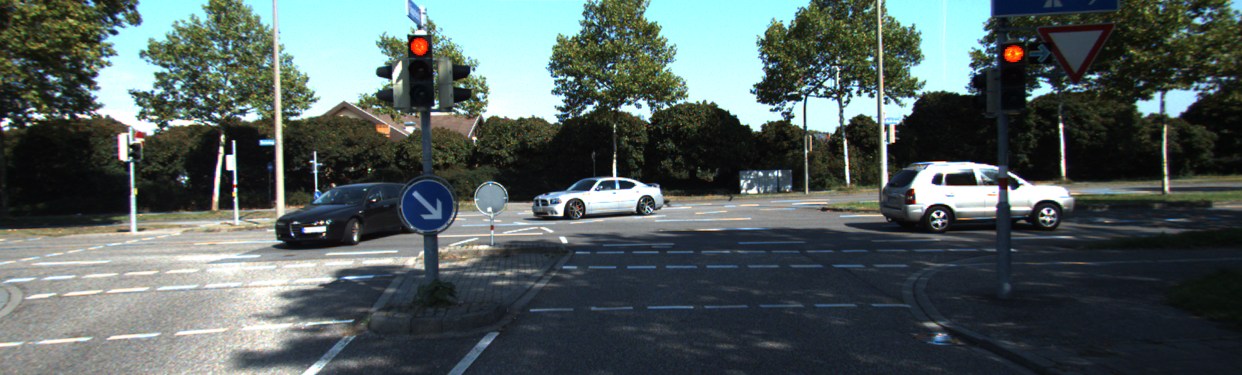
\includegraphics[width=1\linewidth]{figure/kitti_rgb/0000000388.png}\vspace{4pt}
  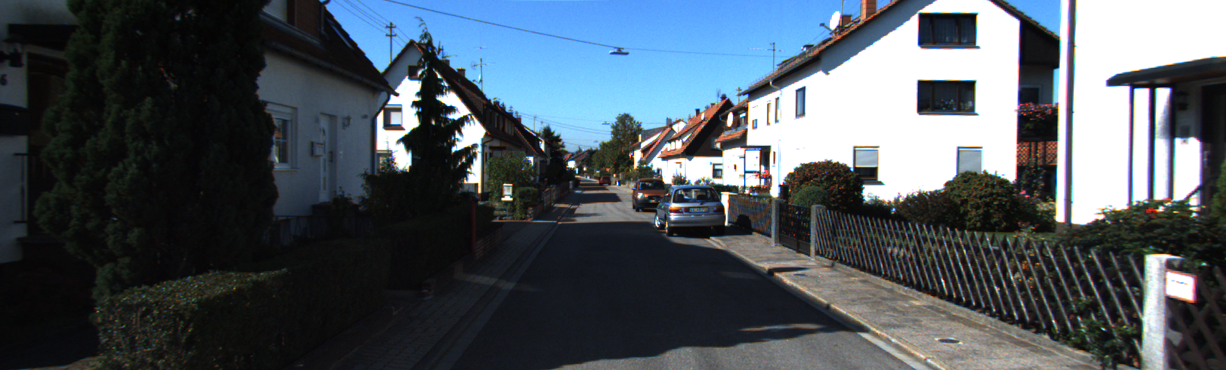
\includegraphics[width=1\linewidth]{figure/kitti_rgb/0000000642.png}
  \end{minipage}
  \caption{RGB图像}
  \end{subfigure}
  \begin{subfigure}{0.15\linewidth}
  \begin{minipage}[b]{1\linewidth}
  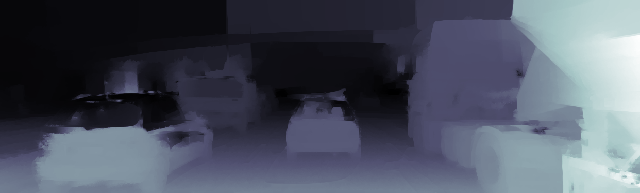
\includegraphics[width=1\linewidth]{figure/kitti_gt/26_52_00.png}\vspace{4pt}
  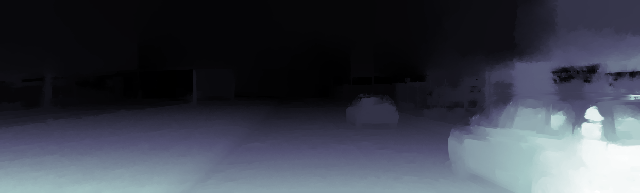
\includegraphics[width=1\linewidth]{figure/kitti_gt/26_13_35.png}\vspace{4pt}
  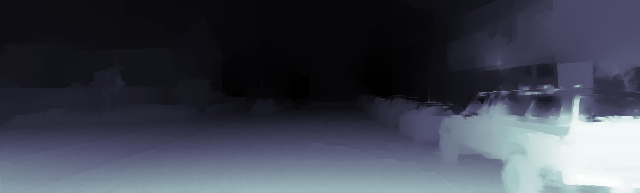
\includegraphics[width=1\linewidth]{figure/kitti_gt/26_09_260.png}\vspace{4pt}
  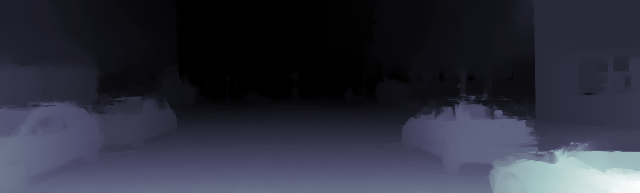
\includegraphics[width=1\linewidth]{figure/kitti_gt/26_09_340.png}\vspace{4pt}
  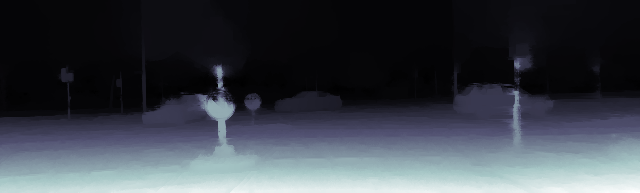
\includegraphics[width=1\linewidth]{figure/kitti_gt/26_09_388.png}\vspace{4pt}
  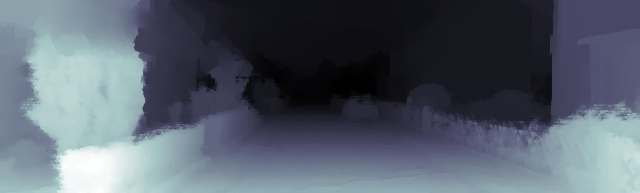
\includegraphics[width=1\linewidth]{figure/kitti_gt/30_18_642.png}
  \end{minipage}
  \caption{真实标注}
  \end{subfigure}
  \begin{subfigure}{0.15\linewidth}
  \begin{minipage}[b]{1\linewidth}
  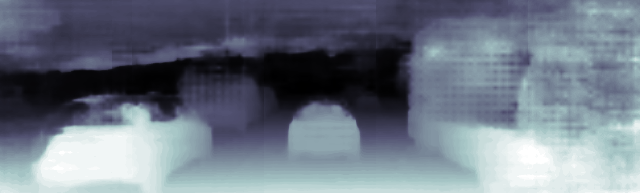
\includegraphics[width=1\linewidth]{figure/dorn/2011_09_26_drive_0052_sync_0000000000.png}\vspace{4pt}
  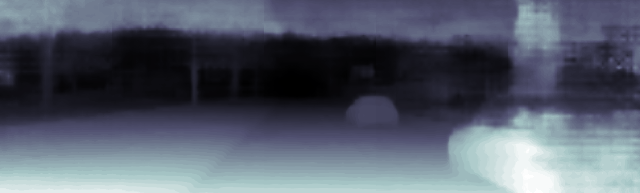
\includegraphics[width=1\linewidth]{figure/dorn/2011_09_26_drive_0013_sync_0000000035.png}\vspace{4pt}
  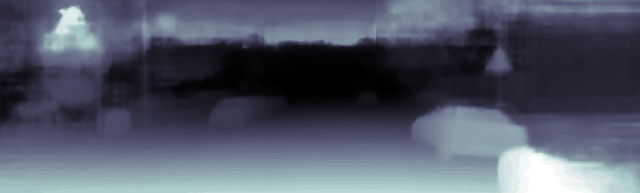
\includegraphics[width=1\linewidth]{figure/dorn/2011_09_26_drive_0009_sync_0000000260.png}\vspace{4pt}
  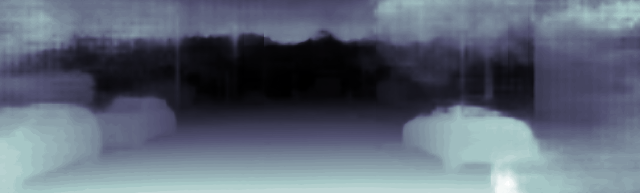
\includegraphics[width=1\linewidth]{figure/dorn/2011_09_26_drive_0009_sync_0000000340.png}\vspace{4pt}
  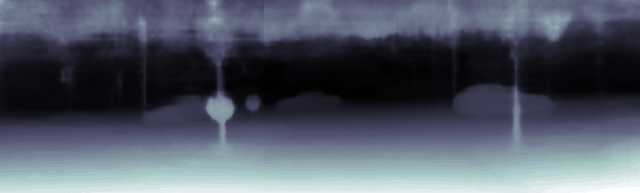
\includegraphics[width=1\linewidth]{figure/dorn/2011_09_26_drive_0009_sync_0000000388.png}\vspace{4pt}
  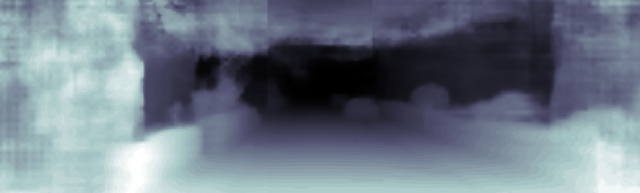
\includegraphics[width=1\linewidth]{figure/dorn/2011_09_30_drive_0018_sync_0000000642.png}
  \end{minipage}
  \caption{DORN~\cite{FuCVPR18-DORN}}
  \end{subfigure}
  \begin{subfigure}{0.15\linewidth}
  \begin{minipage}[b]{1\linewidth}
  
\includegraphics[width=1\linewidth]{figure/kitti_sfm/2011_09_26_drive_0052_sync_0000000000.png}\vspace{3.5pt}
  
\includegraphics[width=1\linewidth]{figure/kitti_sfm/2011_09_26_drive_0013_sync_0000000035.png}\vspace{3.5pt}
  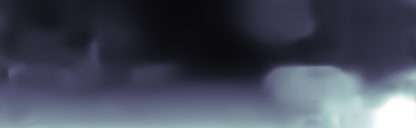
\includegraphics[width=1\linewidth]{figure/kitti_sfm/2011_09_26_drive_0009_sync_0000000260.png}\vspace{3.5pt}
  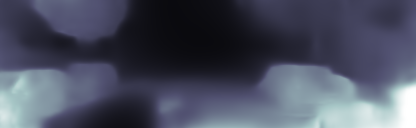
\includegraphics[width=1\linewidth]{figure/kitti_sfm/2011_09_26_drive_0009_sync_0000000340.png}\vspace{3.5pt}
  
\includegraphics[width=1\linewidth]{figure/kitti_sfm/2011_09_26_drive_0009_sync_0000000388.png}\vspace{3.5pt}
  
\includegraphics[width=1\linewidth]{figure/kitti_sfm/2011_09_30_drive_0018_sync_0000000642.png}
  \end{minipage}
  \caption{SfmLearner~\cite{zhou2017unsupervised}}
  \end{subfigure}
  \begin{subfigure}{0.15\linewidth}
  \begin{minipage}[b]{1\linewidth}
  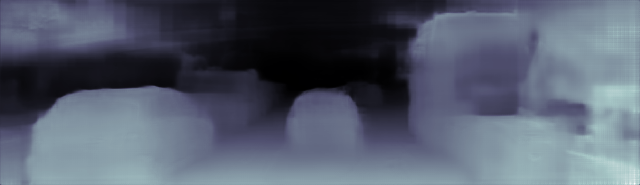
\includegraphics[width=1\linewidth]{figure/kitti_without/2011_09_26_drive_0052_sync_0000000000.png}\vspace{5pt}
  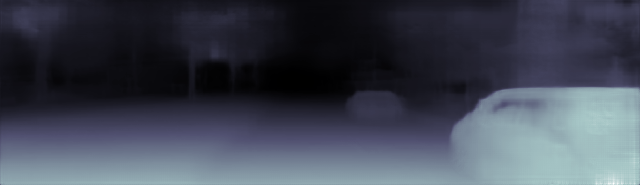
\includegraphics[width=1\linewidth]{figure/kitti_without/2011_09_26_drive_0013_sync_0000000035.png}\vspace{5pt}
  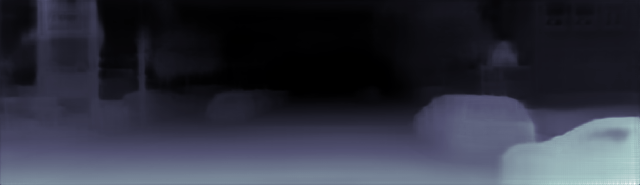
\includegraphics[width=1\linewidth]{figure/kitti_without/2011_09_26_drive_0009_sync_0000000260.png}\vspace{5pt}
  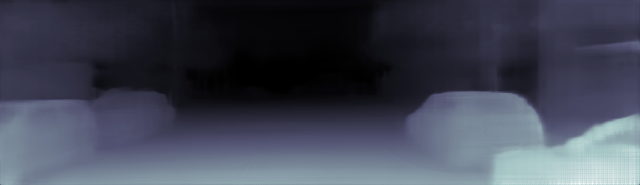
\includegraphics[width=1\linewidth]{figure/kitti_without/2011_09_26_drive_0009_sync_0000000340.png}\vspace{5pt}
  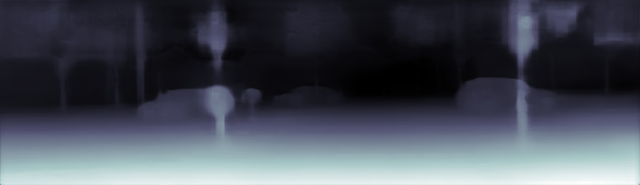
\includegraphics[width=1\linewidth]{figure/kitti_without/2011_09_26_drive_0009_sync_0000000388.png}\vspace{5pt}
  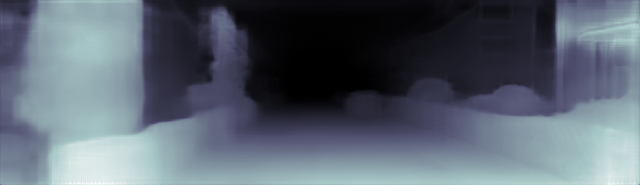
\includegraphics[width=1\linewidth]{figure/kitti_without/2011_09_30_drive_0018_sync_0000000642.png}
  \end{minipage}
  \caption{BTS\cite{bts}}
  \end{subfigure}
  \begin{subfigure}{0.15\linewidth}
  \begin{minipage}[b]{1\linewidth}
  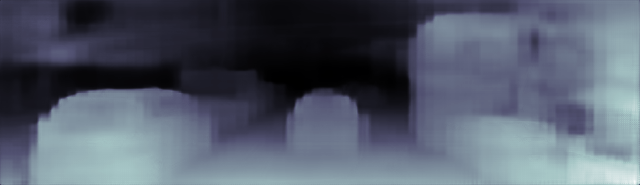
\includegraphics[width=1\linewidth]{figure/kitti_result/2011_09_26_drive_0052_sync_0000000000.png}\vspace{5pt}
  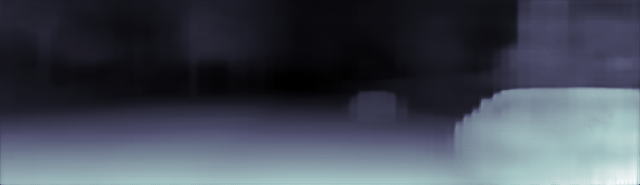
\includegraphics[width=1\linewidth]{figure/kitti_result/2011_09_26_drive_0013_sync_0000000035.png}\vspace{5pt}
  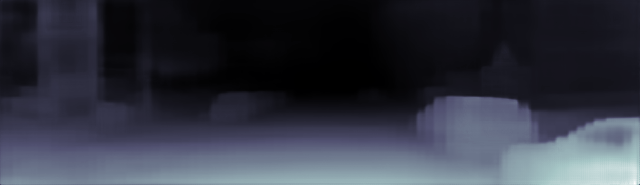
\includegraphics[width=1\linewidth]{figure/kitti_result/2011_09_26_drive_0009_sync_0000000260.png}\vspace{5pt}
  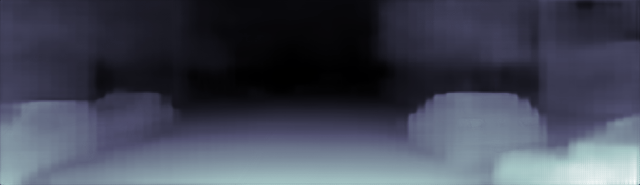
\includegraphics[width=1\linewidth]{figure/kitti_result/2011_09_26_drive_0009_sync_0000000340.png}\vspace{5pt}
  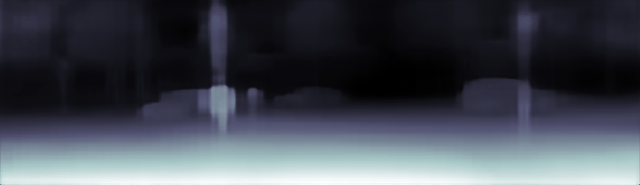
\includegraphics[width=1\linewidth]{figure/kitti_result/2011_09_26_drive_0009_sync_0000000388.png}\vspace{5pt}
  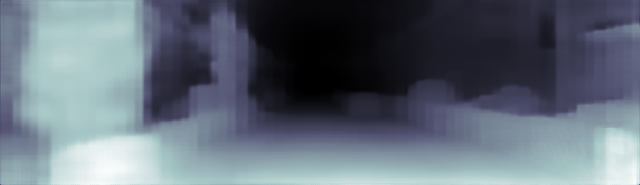
\includegraphics[width=1\linewidth]{figure/kitti_result/2011_09_30_drive_0018_sync_0000000642.png}
  \end{minipage}
  \caption{Ours}
  \end{subfigure}
  \begin{subfigure}{1\linewidth}
    \begin{minipage}[]{0.5\linewidth}
    \centering
     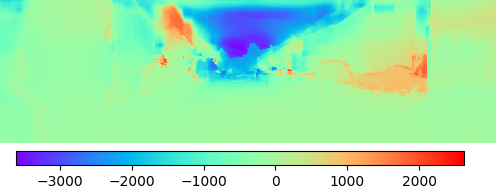
\includegraphics[width=0.95\linewidth]{figure/without_error.png} 
    \end{minipage}
    \begin{minipage}[]{0.5\linewidth}
    \centering
     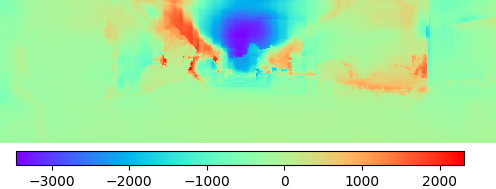
\includegraphics[width=0.95\linewidth]{figure/our_error.png} 
    \end{minipage}
  \end{subfigure}
  \caption{预测结果的可视化对比,对比图中的稀疏真实深度点云使用了
  NYU depth提供的工具箱进行了填充。
  请注意DORN\cite{FuCVPR18-DORN}与SfmLearner\cite{zhou2017unsupervised}
  仅仅使用了KITTI数据集进行了训练,BTS\cite{bts}与本章所用方法
  均使用了复合数据集。热力图为最后一张图像的预测误差图,
  ($map_{error} = D_{gt} - D_{pre}$),左图为BTS\cite{bts}预测误差图,
  右图为本章框架的预测误差图。}
  \label{KITTI visualization result}
  \end{figure*}

实验同样进行了可视化对比。本节展示了与领先方法的视觉效果对比,
如图\ref{KITTI visualization result}所示。相比
DORN\cite{FuCVPR18-DORN}与SfmLearner\cite{zhou2017unsupervised}
本章方法在边界重建和深度精度上都表现良好。
DORN\cite{FuCVPR18-DORN}方法在天空部分预测出现了较大的误差,
而SfmLearner\cite{zhou2017unsupervised}预测的深度图
物体轮廓不够明显。相比BTS\cite{bts},使用本框架时出现了一些锯齿化现象,
这可能是由于添加了自适应池化层造成的。为了更好地展示
框架带来的效果提升,图\ref{KITTI visualization result}
最后一行展示了放大的预测误差图。图左为最后一张RGB图像
使用BTS在复杂数据集训练后预测深度图的误差图,图右为
使用自蒸馏框架在复杂数据集训练后预测深度图的误差图,可以
本章提出的自蒸馏框架对效果有着明显的提升。可以发现自蒸馏框架的加入
使得网络在远距离的预测误差(蓝色区域)大幅减少。

NYU数据集上的视觉对比如图\ref{nyu visualization result}所示,
自蒸馏框架在细节的预测上表现优异,如第一幅图像中的书架,
第四幅图中的人像,
第五幅图像中的浴缸等。

\subsection{算法复杂度分析}
本节重点分析该自蒸馏框架的时间与空间复杂度,以
验证该系统后续在线使用的可能性。由于框架适用于大多数
编解码网络,所以框架实际复杂度与所采用的编解码结构有关,
本节分析
了使用BTS\cite{bts}作为编解码结构的自蒸馏框架复杂度。本实验
采用了四张英伟达2080TI显卡,
Intel(R) Xeon(R) CPU E5-2678 v3 @ 2.50GHz cpu
来搭建硬件实验平台。软件方面,使用了英伟达418.56
版本驱动,CUDA使用了10.1版本,pytorch使用了1.1.0版本来进行
算法实现。
在训练时间上,该框架经过了学生编码器和负学生编码器的两次前项推理和
一次反向传播过程,完成一个训练周期,共计46672张图像训练
耗时3.12h,平均每张图片耗时0.24s。在推理阶段,
平均每张图片耗时0.09s。每次迭代自蒸馏框架浮点运算量
为1.18TFLOPs。在空间复杂度上,自蒸馏框架共计73848300个参数
其中可训练参数为73790040个,但是由于自蒸馏框架在推理阶段不需要
负学生编码器,所以只有47000688个参数。

\begin{figure*}[htb]
  \centering
  \begin{subfigure}{0.15\linewidth}
    
  \begin{minipage}[t]{1\linewidth}
  \centering
  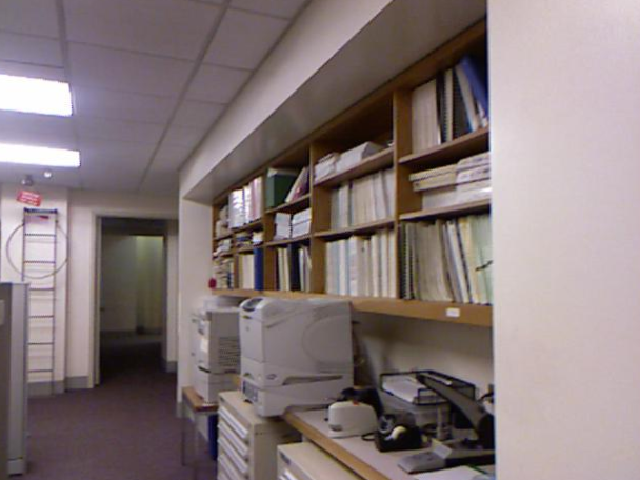
\includegraphics[width=1\linewidth]{figure/nyu_rgb/15.png}
  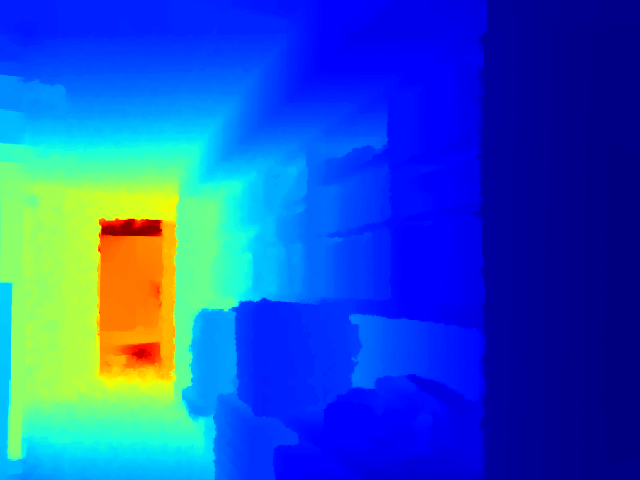
\includegraphics[width=1\linewidth]{figure/nyu_gt/15.png}
  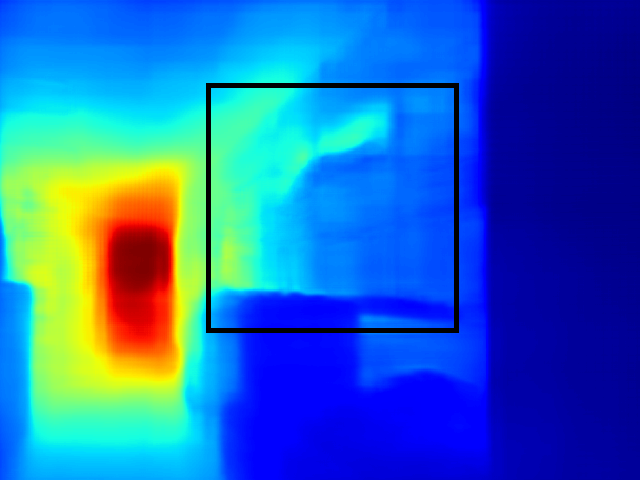
\includegraphics[width=1\linewidth]{figure/nyu_result/office_rgb_00015.png}
  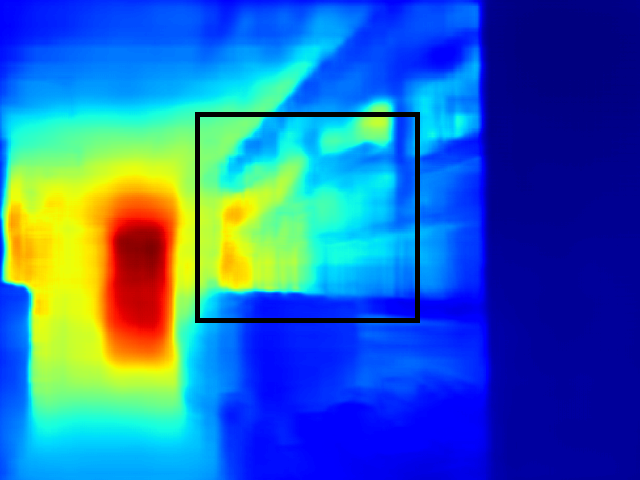
\includegraphics[width=1\linewidth]{figure/nyu_without/office_rgb_00015.png}
  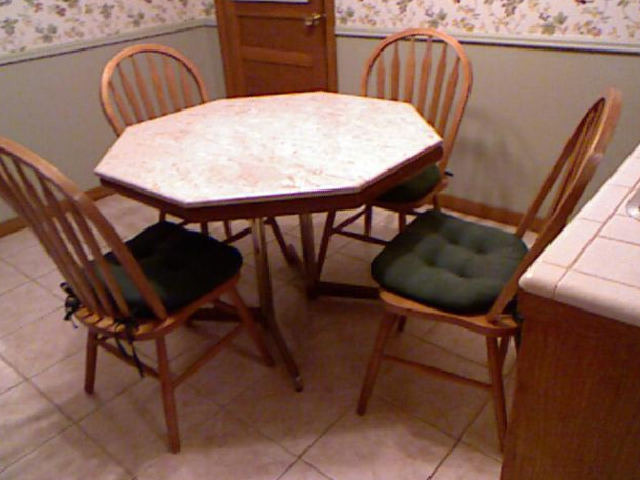
\includegraphics[width=1\linewidth]{figure/nyu_rgb/760.png}
  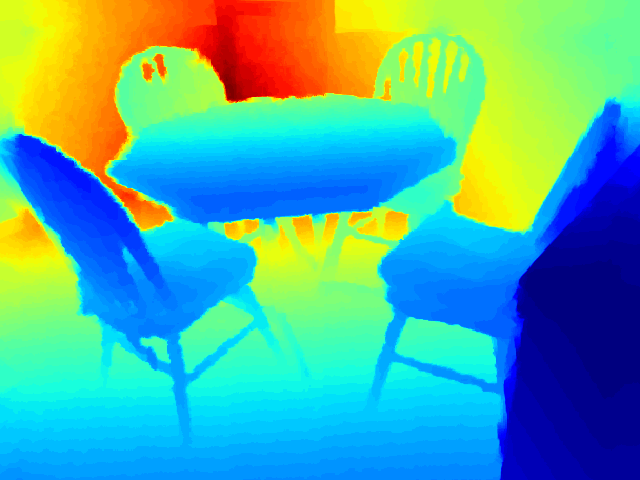
\includegraphics[width=1\linewidth]{figure/nyu_gt/760.png}
  \includegraphics[width=1\linewidth]{figure/nyu_result/kitchen_rgb_00760.png}
  \includegraphics[width=1\linewidth]{figure/nyu_without/kitchen_rgb_00760.png}
  %\caption{fig1}
  \end{minipage}%
  
  \end{subfigure}
  \begin{subfigure}{0.15\linewidth}
    
  \begin{minipage}[t]{1\linewidth}
  \centering
  \includegraphics[width=1\linewidth]{figure/nyu_rgb/170.png}
  \includegraphics[width=1\linewidth]{figure/nyu_gt/170.png}
  \includegraphics[width=1\linewidth]{figure/nyu_result/bedroom_rgb_00170.png}
  \includegraphics[width=1\linewidth]{figure/nyu_without/bedroom_rgb_00170.png}
  \includegraphics[width=1\linewidth]{figure/nyu_rgb/850.png}
  \includegraphics[width=1\linewidth]{figure/nyu_gt/850.png}
  \includegraphics[width=1\linewidth]{figure/nyu_result/kitchen_rgb_00850.png}
  \includegraphics[width=1\linewidth]{figure/nyu_without/kitchen_rgb_00850.png}
  %\caption{fig2}
  \end{minipage}%
  \end{subfigure}
  \begin{subfigure}{0.15\linewidth}
    
  \begin{minipage}[t]{1\linewidth}
  \centering
  \includegraphics[width=1\linewidth]{figure/nyu_rgb/431.png}
  \includegraphics[width=1\linewidth]{figure/nyu_gt/431.png}
  \includegraphics[width=1\linewidth]{figure/nyu_result/playroom_rgb_00431.png}
  \includegraphics[width=1\linewidth]{figure/nyu_without/playroom_rgb_00431.png}
  \includegraphics[width=1\linewidth]{figure/nyu_rgb/1078.png}
  \includegraphics[width=1\linewidth]{figure/nyu_gt/1078.png}
  \includegraphics[width=1\linewidth]{figure/nyu_result/bedroom_rgb_01078.png}
  \includegraphics[width=1\linewidth]{figure/nyu_without/bedroom_rgb_01078.png}
  %\caption{fig2}
  \end{minipage}%
  \end{subfigure}
  \begin{subfigure}{0.15\linewidth}
    
  \begin{minipage}[t]{1\linewidth}
  \centering
  \includegraphics[width=1\linewidth]{figure/nyu_rgb/566.png}
  \includegraphics[width=1\linewidth]{figure/nyu_gt/566.png}
  \includegraphics[width=1\linewidth]{figure/nyu_result/kitchen_rgb_00566.png}
  \includegraphics[width=1\linewidth]{figure/nyu_without/kitchen_rgb_00566.png}
  \includegraphics[width=1\linewidth]{figure/nyu_rgb/1149.png}
  \includegraphics[width=1\linewidth]{figure/nyu_gt/1149.png}
  \includegraphics[width=1\linewidth]{figure/nyu_result/bedroom_rgb_01149.png}
  \includegraphics[width=1\linewidth]{figure/nyu_without/bedroom_rgb_01149.png}
  %\caption{fig2}
  \end{minipage}%
  \end{subfigure}
  \begin{subfigure}{0.15\linewidth}
    
  \begin{minipage}[t]{1\linewidth}
  \centering
  \includegraphics[width=1\linewidth]{figure/nyu_rgb/668.png}
  \includegraphics[width=1\linewidth]{figure/nyu_gt/668.png}
  \includegraphics[width=1\linewidth]{figure/nyu_result/bathroom_rgb_00668.png}
  \includegraphics[width=1\linewidth]{figure/nyu_without/bathroom_rgb_00668.png}
  \includegraphics[width=1\linewidth]{figure/nyu_rgb/1313.png}
  \includegraphics[width=1\linewidth]{figure/nyu_gt/1313.png}
  \includegraphics[width=1\linewidth]{figure/nyu_result/living_room_rgb_01313.png}
  \includegraphics[width=1\linewidth]{figure/nyu_without/living_room_rgb_01313.png}
  %\caption{fig2}
  \end{minipage}%
  \end{subfigure}
  \begin{subfigure}{0.15\linewidth}
    
  \begin{minipage}[t]{1\linewidth}
  \centering
  \includegraphics[width=1\linewidth]{figure/nyu_rgb/706.png}
  \includegraphics[width=1\linewidth]{figure/nyu_gt/706.png}
  \includegraphics[width=1\linewidth]{figure/nyu_result/bathroom_rgb_00706.png}
  \includegraphics[width=1\linewidth]{figure/nyu_without/bathroom_rgb_00706.png}
  \includegraphics[width=1\linewidth]{figure/nyu_rgb/1399.png}
  \includegraphics[width=1\linewidth]{figure/nyu_gt/1399.png}
  \includegraphics[width=1\linewidth]{figure/nyu_result/dining_room_rgb_01399.png}
  \includegraphics[width=1\linewidth]{figure/nyu_without/dining_room_rgb_01399.png}
  %\caption{fig2}
  \end{minipage}%
  \end{subfigure}
  \centering
  \caption{使用复合数据集训练在NYU数据集上预测的表现对比:
   第一行RGB图像,第二行真实标注,第三行为使用自蒸馏框架训练的预测结果,
   第四行为使用常规训练的预测结果。}
  \label{nyu visualization result}
  \end{figure*}
%%%%%%%%%%%%%%%%%%%%%%%%%%%%%%%%%%%%%%%%%%%%%%%%%%%%%%%%%%%%%%%%%%%%%%%
\section{本章小结}
本章关注到单目深度估计网络的鲁棒性问题,即面对各种复杂场景的稳定性问题,
使用深度学习的方法解决鲁棒性问题可以简单地扩大数据集,在数量和多样性
上对数据集进行丰富。在将室内数据集NYU depth v2与
室外数据集KITTI进行组合以丰富数据集并进行训练以后,
一个新的问题暴露出来:两种方法Li\cite{DABC}和BTS
\cite{bts}在这种复杂数据集上的表现都有了不同程度的退化。
这是由于使用一个网络难以去拟合两个完全不同的数据分布。即
符复杂多样的数据分布对网络的拟合能力和表达能力提出了更高的要求。
为了解决这个问题,本章提出了一种自蒸馏单目深度估计网络。
一方面自蒸馏单目深度估计网络通过学生编码器和解码器学习
深度估计的映射,另一方面,通过负学生编码器提取负样本特征,并使用
余弦相似性来惩罚两种特征,使得两种特征在特征空间的距离逐渐扩大。
即编码器会针对两种数据集提取两种具有明显差异的特征,以此来
使网络对复杂场景进行区分。实验表明自蒸馏单目深度估计网络
极大地提升了网络的拟合能力与表达能力。对比实验说明该框架
一定程度上减弱了这种退化现象,甚至使得某些指标超过了面对单一数据集
时的表现。视觉对比实验表明框架在预测精确度,边缘重建,
细节预测上均比使用常规的训练方法更优秀。





